\input texbase

\titulo{Exercício Programa 1}
\materia{MAC5915 - Laboratório de Visão Computacional e Processamento de Imagens}

\aluno{Fernando Omar Aluani}{6797226}

\begin{document}
\cabecalho

%===================================================================================
\section{Introdução}
Esse relatório apresenta a minha implementação desse exercício-programa, que
consiste na implementação (não exata) do algoritmo de detecção de placas veiculares
descrita no artigo dado: ``\textit{An efficient method of license plate location}'' de Zheng et al.

Irei começar com uma revisada simples do algoritmo ``oficial'' (do artigo), para depois descrever
minha implementação e suas diferenças com o original, e finalmente apresentar alguns resultados.

%===================================================================================
\section{Algoritmo de Detecção de Placas}
O artigo descreve que testou o algoritmo com bases de dados de imagens com $384 x 288$ pixels, em
escala de cinza. 

O algoritmo em si consiste de 4 etapas, partindo da imagem original:
\begin{enumerate}
  \item \textbf{Melhoramento da Imagem}: consiste em tentar ``melhorar'' a imagem para balancear
    os contrastes e realçar a placa.
  \item \textbf{Extração de Arestas Verticais}: consiste em adquirir a imagem gradiente vertical
    com Sobel, depois binarizar o gradiente com algum limite e aplicar supressão de não-máximos.    
  \item \textbf{Remoção de Ruído e Curvas do Fundo}: consiste em aplicar um algoritmo próprio
    (descrito no artigo) para remover arestas verticais muito longas (que não seriam parte da placa,
    usualmente são parte de objetos do fundo) e muito curtas (ruído que também não é parte da placa).
  \item \textbf{Segmentação e Busca da Placa}: consiste em passar uma janela na imagem de arestas 
    para achar a localização da placa.
\end{enumerate}

Os valores de limite para arestas longas e curtas, e tamanho da janela para localização das placas são
parâmetros do algoritmo mas são dados como valores estáticos, sendo que o valor otimal para tais parâmetros
podem mudar entre imagems de placas diferentes.

%===================================================================================
\section{Implementação}
% descrição do que foi implementado
Minha implementação segue o formato de quatro etapas do algoritmo original, cada uma operando sobre
o resultado da anterior. Porém na implementação de cada etapa alterei alguns detalhes, como explicado
nas subseções a seguir.

%--------------------------------------------------------------------------------
\subsection{Melhoramento da Imagem}
Nessa etapa, só há duas grandes diferenças. A primeira é que a minha implementação usa imagens integrais
para executar os cálculos de soma e desvio padrão de áreas da imagem, o que simplifica o código e aumenta
sua eficiência.

A segunda diferença é que fiz essa etapa ser opcional (por padrão não é executada). Pelos meus testes com
a base de dados, a diferença da imagem original para a imagem melhorada é pouca e praticamente não
afetava o resultado final da detecção da placa.

%--------------------------------------------------------------------------------
\subsection{Extração de Arestas Verticais}
Usei método pronto do OpenCV para executar o operador Sobel vertical (com matriz $3x3$), e então rodo
módulo na imagem gradiente para todos valores serem positivos. Depois também uso um método de binarização
(\textit{thresholding}) do OpenCV para binarizar o gradiente usando o \textit{threshold} de Otsu.

Finalmente aplico a supressão de não-máximos no sentido horizontal usando um algoritmo que implementei.

%--------------------------------------------------------------------------------
\subsection{Remoção de Ruído e Curvas do Fundo}
Essa etapa implementei o mesmo algoritmo descrito no artigo, com a exceção que fiz os parâmetros de limite
de arestas longas e curtas poderem ser passados pelo usuário. Dessa forma podemos executar o mesmo programa
para imagens diferentes só alterando os parâmetros. Por padrão deixei os mesmos valores que são dados no artigo.

%--------------------------------------------------------------------------------
\subsection{Segmentação e Busca da Placa}
Nessa etapa eu ainda passo uma janela pela imagem para achar a região com maior concentração de arestas
verticais, mas em vez de usar o algoritmo dado no artigo eu simplesmente usei imagens integrais.
Também deixei o tamanho (altura e largura) da janela ser passado pelo usuário. 

%===================================================================================
\section{Resultados}
% ilustrações dos resultados para algumas imagens e os tempos de execução
\subsection{Programa}
O programa e a implementação do algoritmo está todo contido em um script \emph{Python}:
\textbf{placas.py}. Ele pode:
\begin{itemize}
  \item ser executado como um script na linha de comando para buscar a placa de uma imagem. 
    Nesse caso, executando-o sem argumentos ou passando \textbf{--help} ou \textbf{-h} irá
    imprimir uma descrição completa de como rodar o programa e quais são seus possíveis argumentos.
  \item ser importado como um módulo \emph{python} em outro \textit{script}. Nesse caso o outro \textit{script}
    poderá usar a classe de imagem integral e executar as funções correspondentes aos passos.
\end{itemize}

Para executar o \textit{script} é necessário \emph{python} versão $2.7$ ou mais, OpenCV (para \emph{python})
e \emph{NumPy} instalados. Essas bibliotecas são fáceis de encontrar e instalar em várias plataformas. 
Particularmente, para que a opção \textbf{--display} funcione, a biblioteca \emph{PyLab} (que contém
\emph{NumPy}, \emph{SciPy} e \emph{Matplotlib}) também precisa estar instalada.

\subsection{Execuções}

As seguintes imagens mostram o resultado visual de comparação das etapas do algoritmo, gerado pelo programa.
Todas foram executadas com os valores padrão de argumentos.

A figura \ref{errado} mostra um teste que falhou. Ele rodou sem a etapa de melhoramento.
\begin{figure}
  \centering
  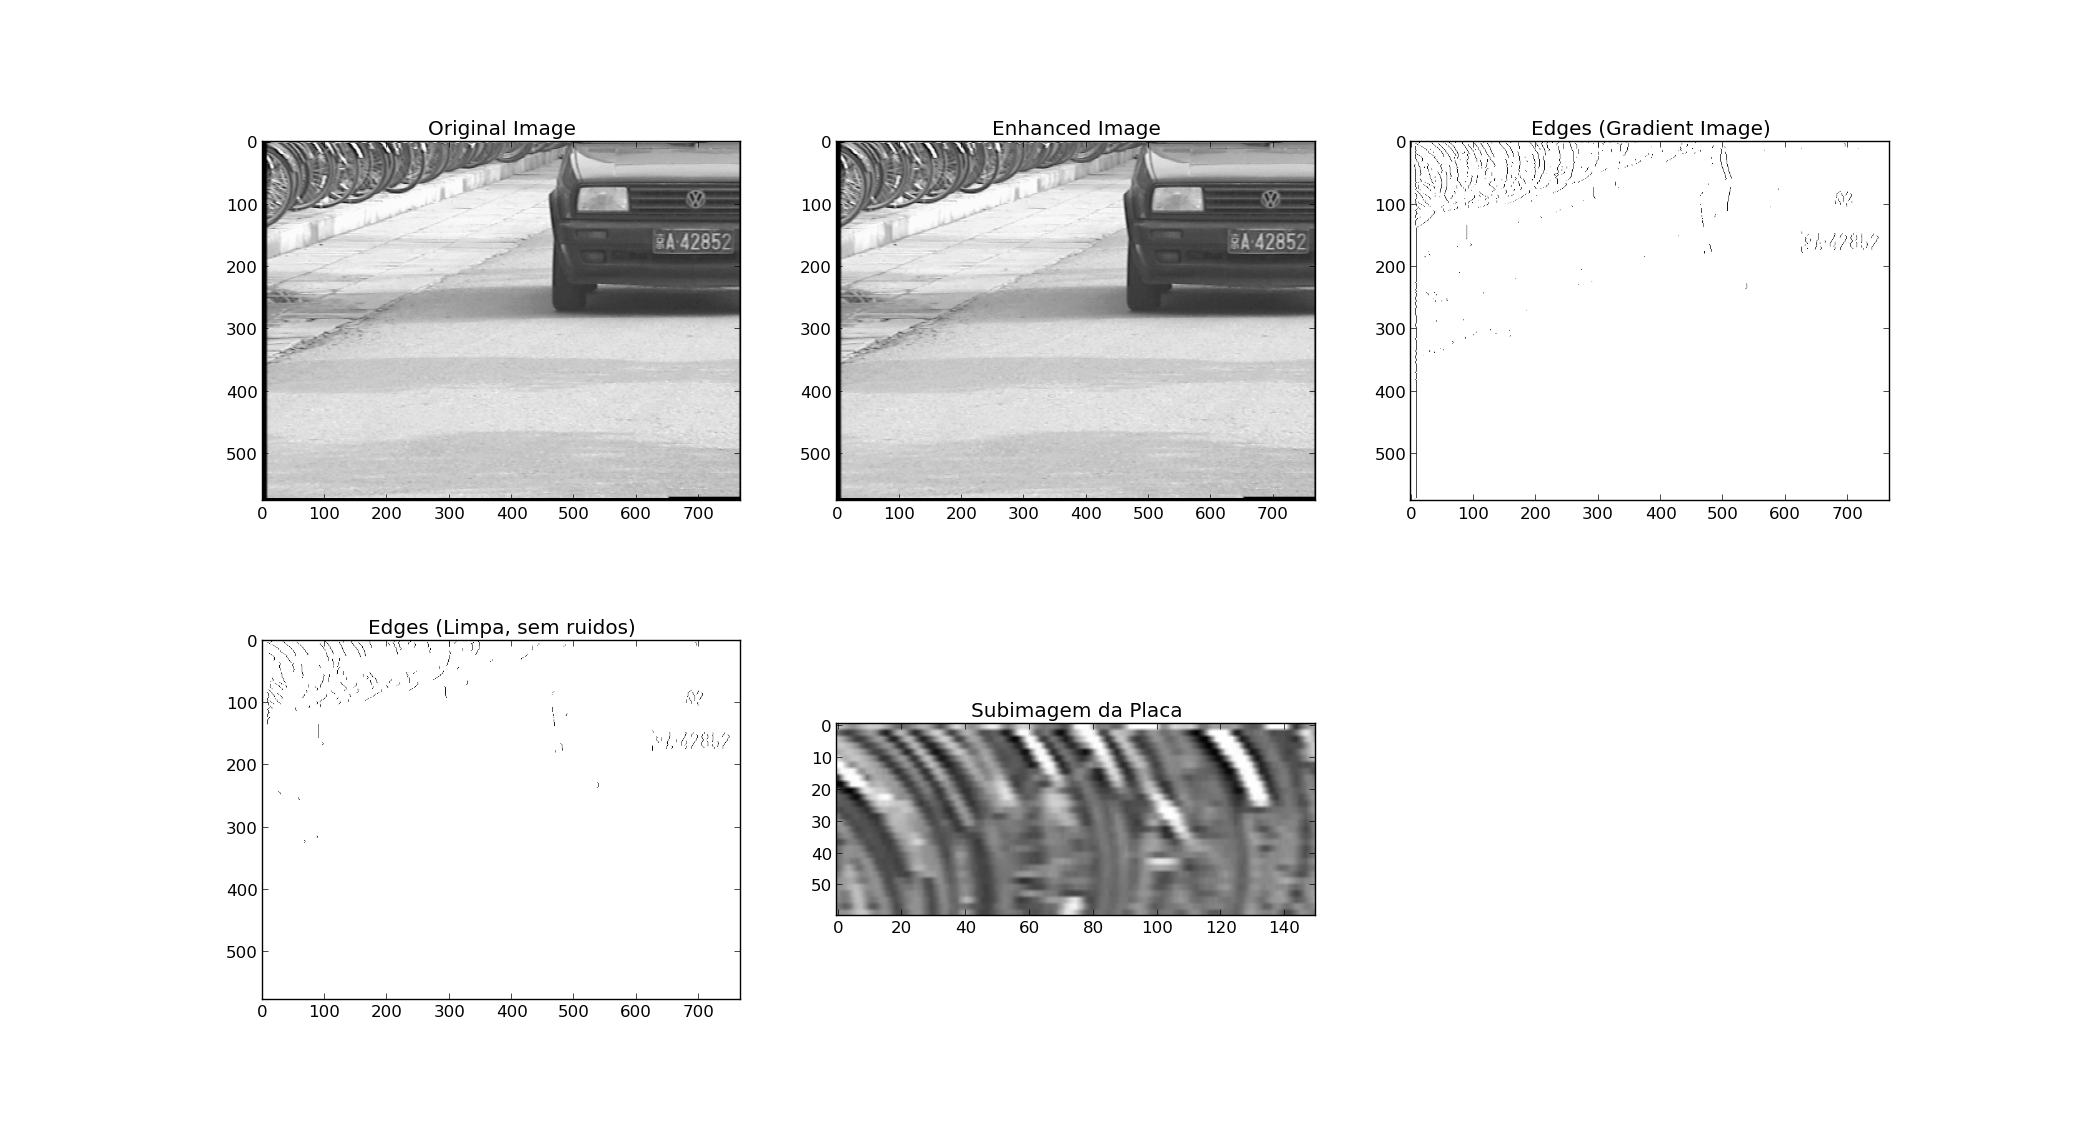
\includegraphics[clip=true, trim=185 20 150 20, scale=0.4]{errado.png}
  \caption{Teste que falhou.}
  \label{errado}
\end{figure}

A figura \ref{duasplacas} mostra um teste (sem etapa de melhoramento) no qual há duas placas na imagem, e ele consegue achar a correta.
\begin{figure}
  \centering
  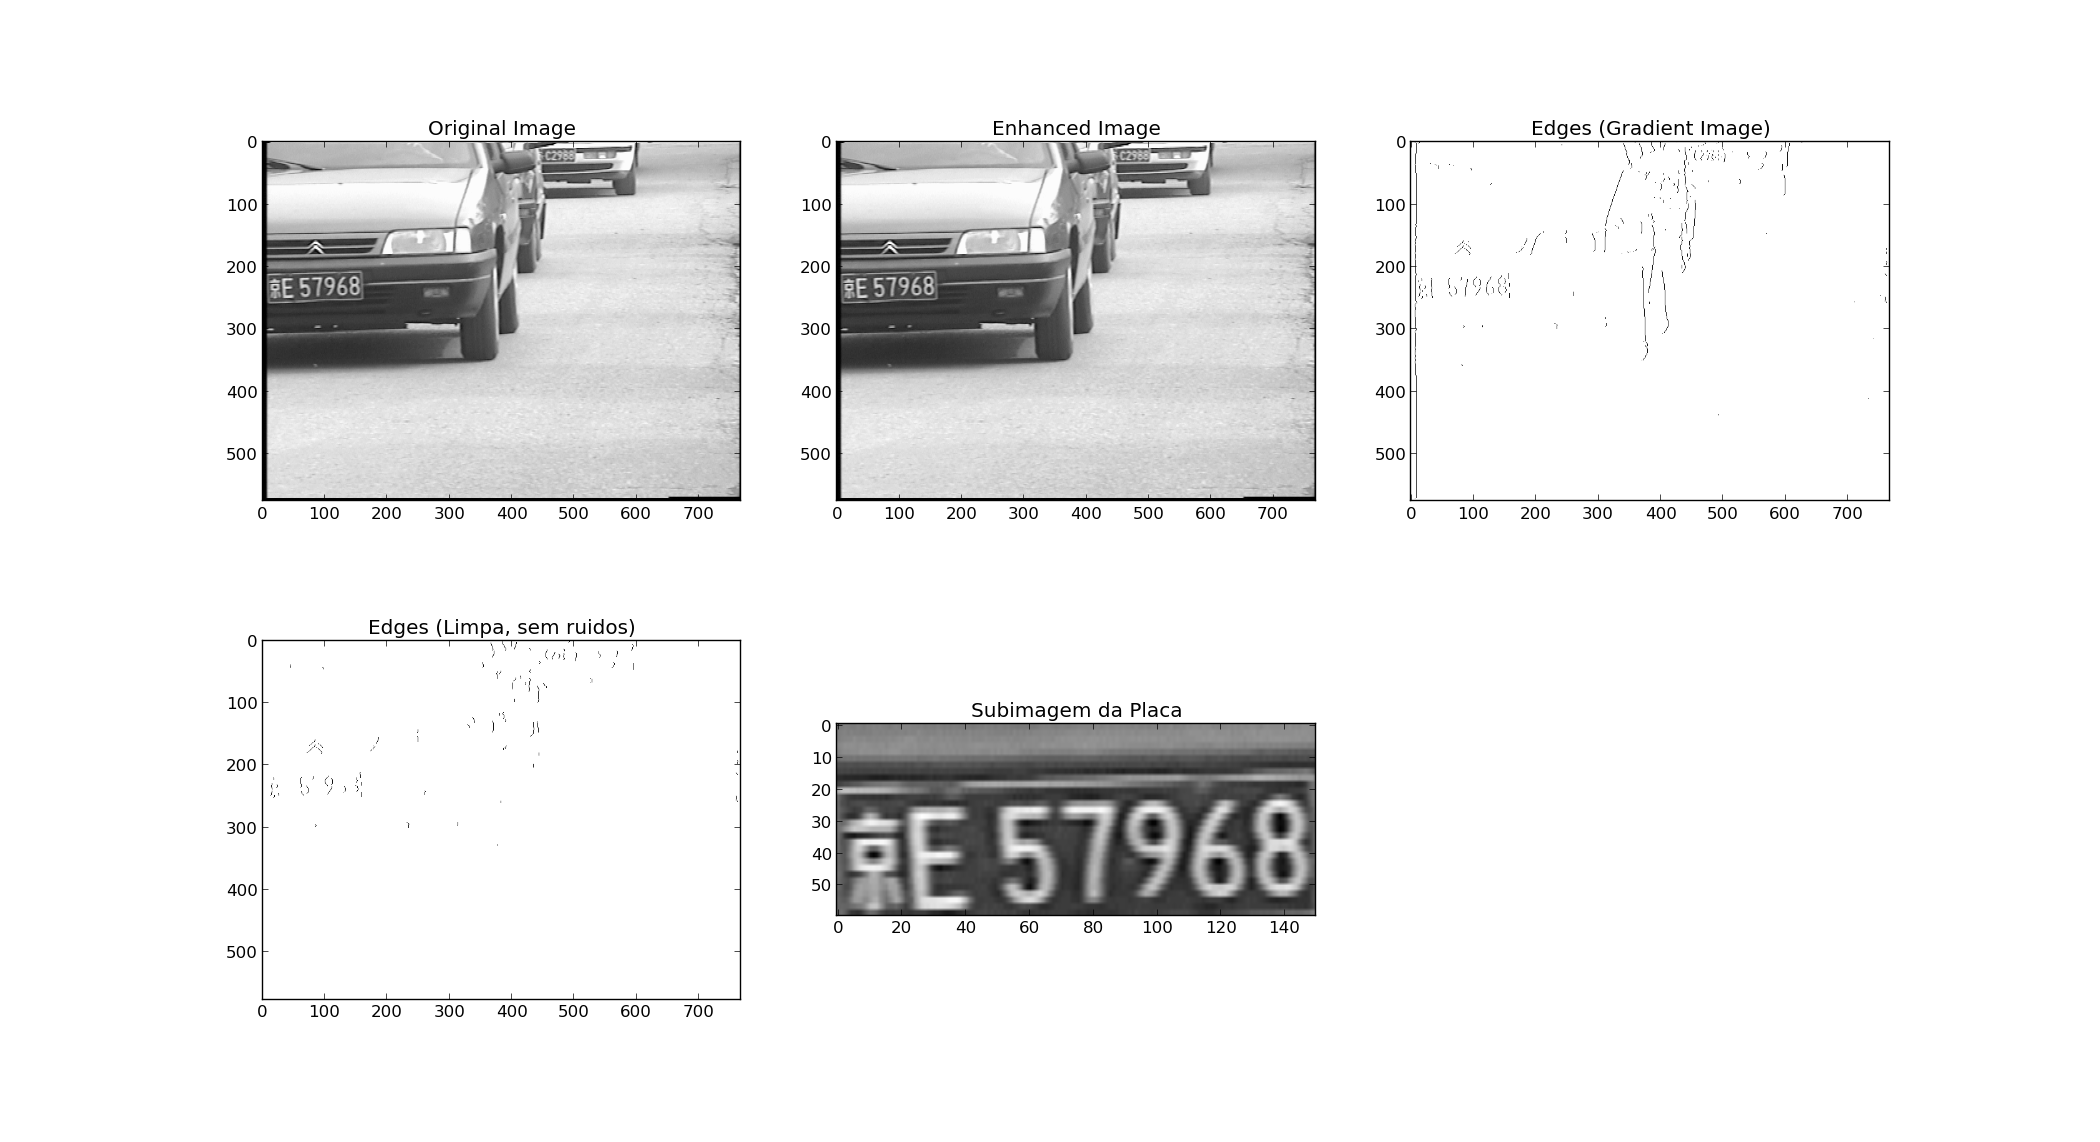
\includegraphics[clip=true, trim=185 20 150 20, scale=0.4]{duasPlacasCerto.png}
  \caption{Teste com duas placas na imagem, achando a correta.}
  \label{duasplacas}
\end{figure}

A figura \ref{comenhance} mostra um teste bem sucedido com a etapa de melhoramento, enquanto
a figura \ref{semenhance} mostra o mesmo teste mas sem essa etapa. Ambos foram bem sucedidos, com
uma diferença bem pequena no resultado, enquanto o tempo de execução sem a etapa de melhoramento é 
bem mais rápido.
\begin{figure}
  \centering
  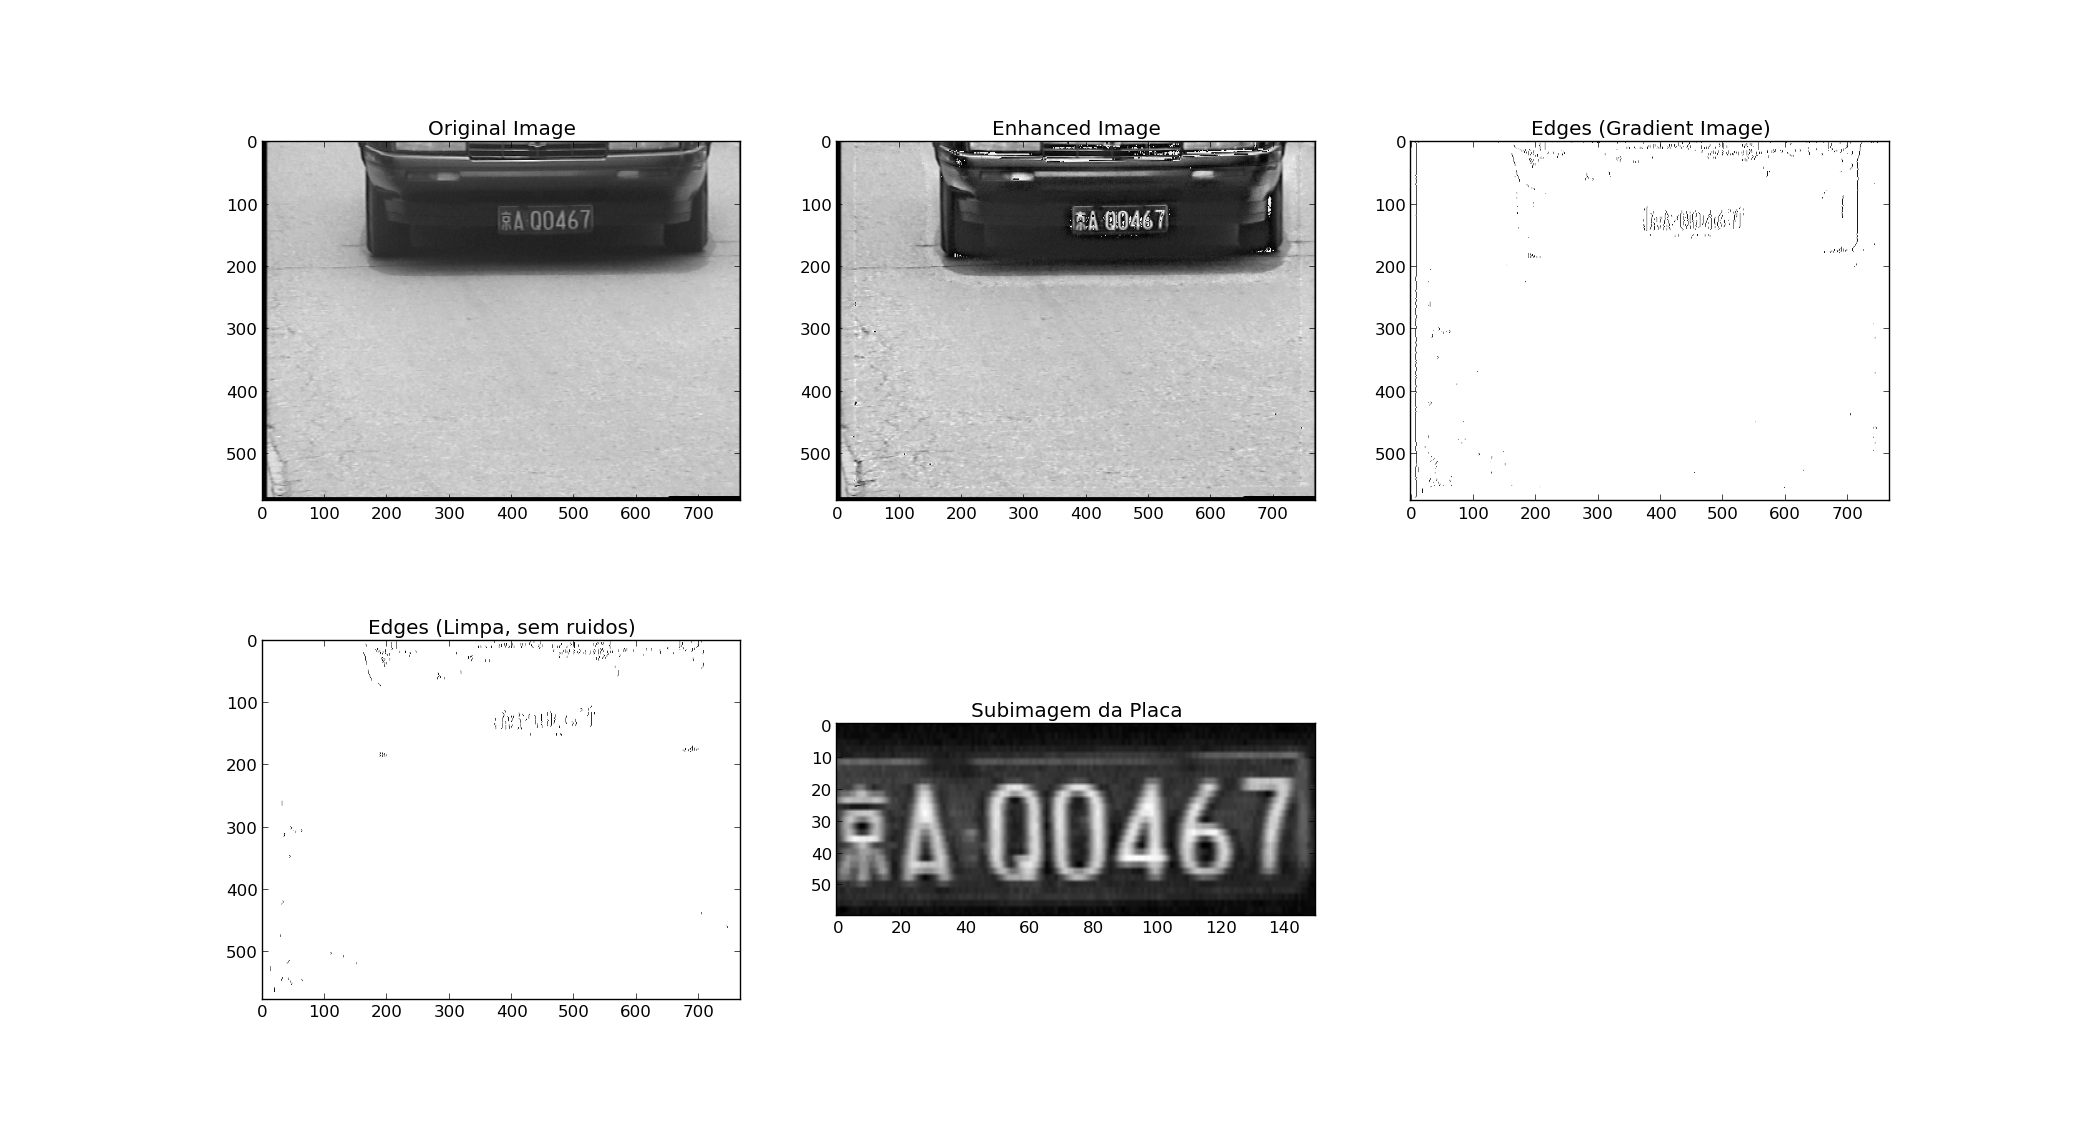
\includegraphics[clip=true, trim=185 20 150 20, scale=0.4]{displayComEnhance.png}
  \caption{Teste com etapa de melhoramento.}
  \label{comenhance}
\end{figure}

\begin{figure}
  \centering
  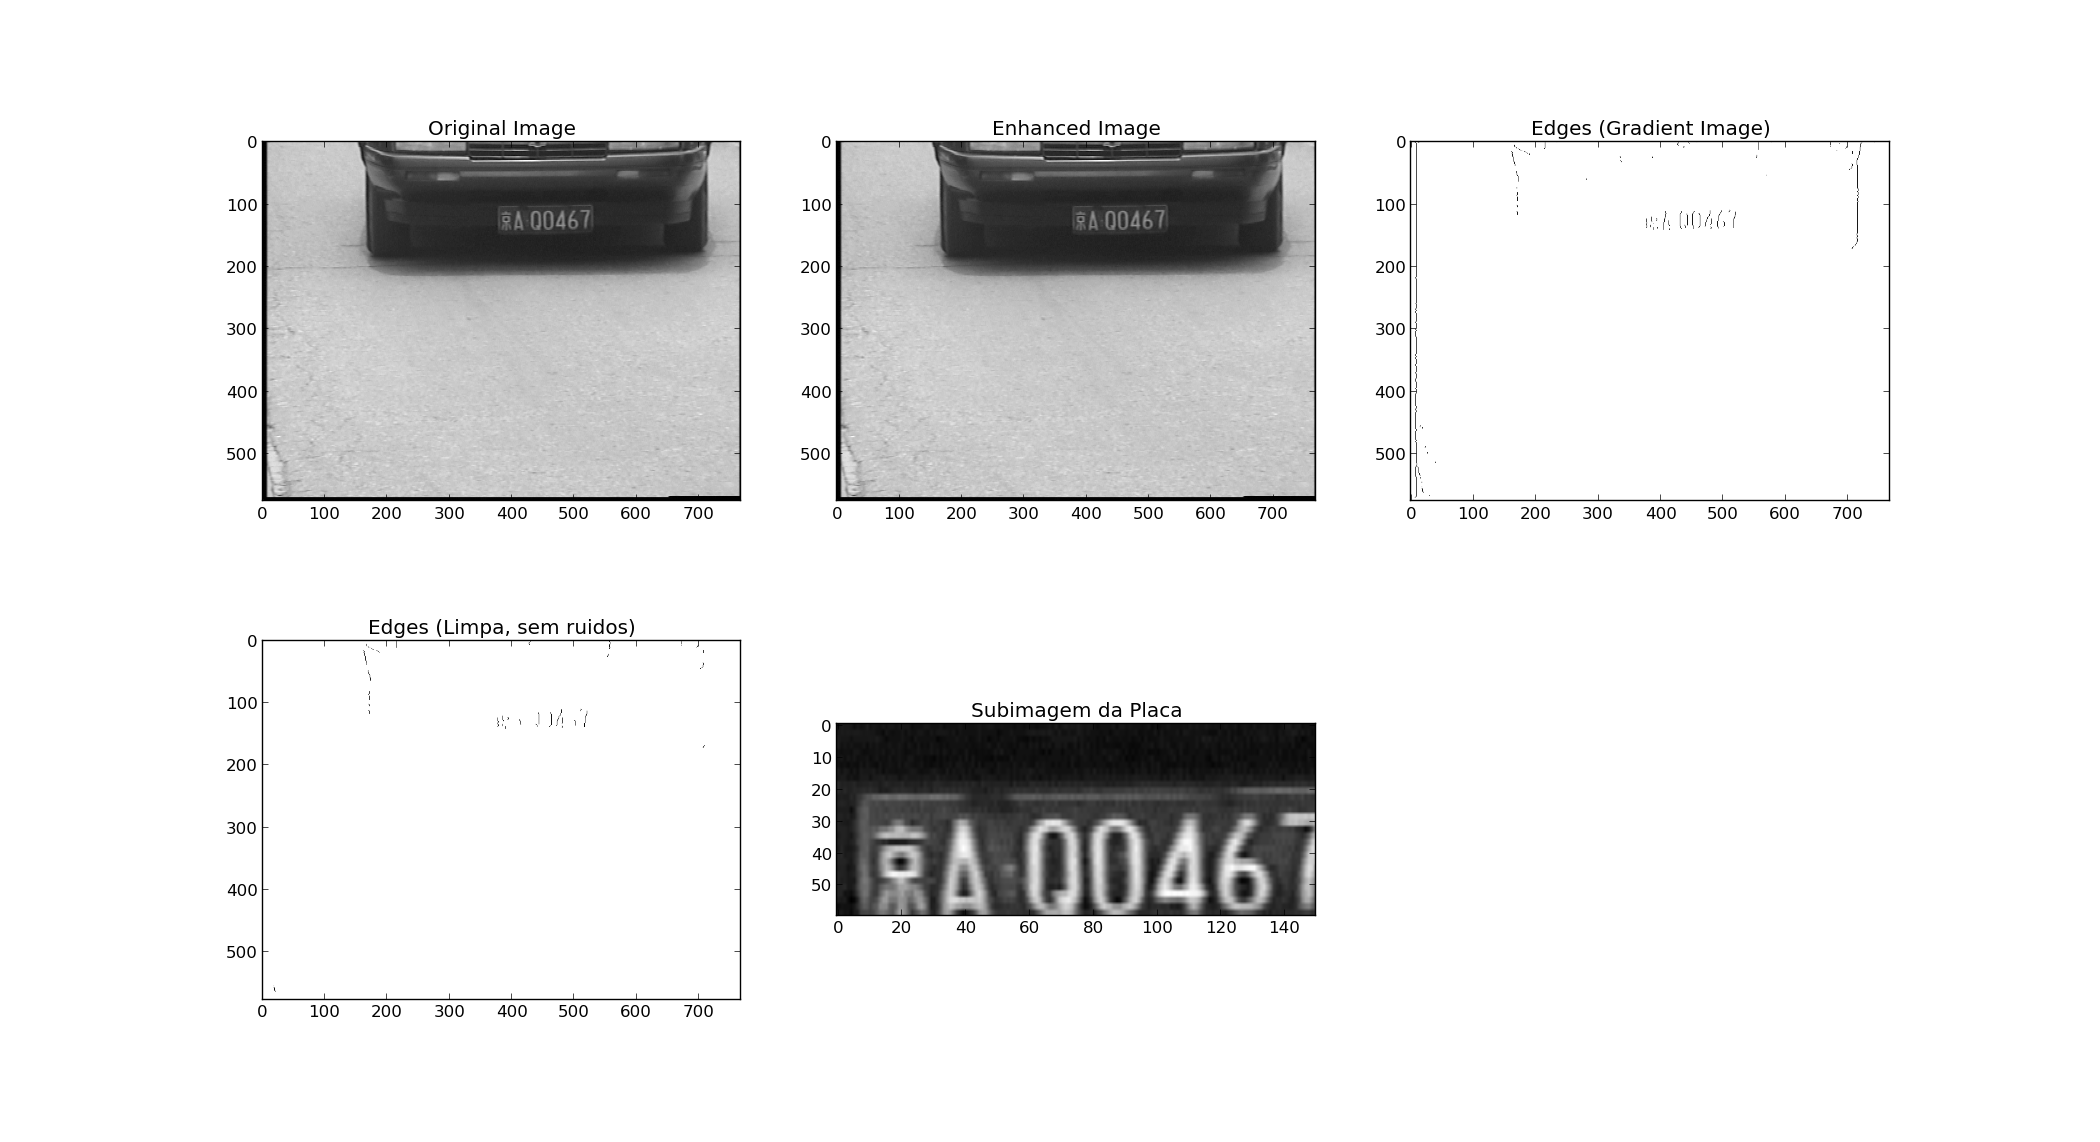
\includegraphics[clip=true, trim=185 20 150 20, scale=0.4]{displaySemEnhance.png}
  \caption{Mesmo teste anterior, mas sem etapa de melhoramento.}
  \label{semenhance}
\end{figure}

\subsubsection{Tempos de execução}
\begin{tabular}{ | l | c | c | c | c | c | r | }
\hline
Teste       & Leitura & Etapa 1 & Etapa 2 & Etapa 3 & Etapa 4 & Total \\
\hline
\ref{errado} & 0.08 & N/A & 5.19 & 10.00 & 8.24 & 23.51 \\
\hline
\ref{duasplacas} & 0.07 & N/A & 4.85 & 9.30 & 8.01 & 22.23 \\
\hline
\ref{comenhance} & 0.07 & 31.41 & 4.52 & 8.86 & 8.86 & 53.73 \\
\hline
\ref{semenhance} & 0.0 & N/A & 4.38 & 8.73 & 7.59 & 20.70 \\
\hline
\end{tabular}

\end{document}
